% ============================================================================
%  Verification of a Local VQE Stack for a Thio-Michael Addition,
%  and the Cost Boundary of Simulating It
%
%  Compile:  pdflatex main.tex     (run three times: ToC + cross-references)
%  No bibtex pass required -- the bibliography is inline.
%  Figures expected in ./figures/
% ============================================================================
\documentclass[11pt,a4paper]{article}

\usepackage[T1]{fontenc}
\usepackage[utf8]{inputenc}
\usepackage{lmodern}
\usepackage[margin=2.4cm,headheight=14pt]{geometry}
\usepackage{amsmath,amssymb}
\usepackage{graphicx}
\usepackage{booktabs}
\usepackage{array}
\usepackage{caption}
\usepackage{enumitem}
\usepackage{fancyhdr}
\usepackage{microtype}
\usepackage{xcolor}

\definecolor{NavyLink}{HTML}{1A4C8B}
\definecolor{BoxBlue}{HTML}{EAF1F9}
\definecolor{BoxRule}{HTML}{1A4C8B}
\definecolor{WarnBg}{HTML}{FDF3E7}
\definecolor{WarnRule}{HTML}{9C5B12}
\definecolor{StopBg}{HTML}{F5EEEE}
\definecolor{StopRule}{HTML}{8B1A1A}

\usepackage{tcolorbox}
\usepackage[colorlinks=true,linkcolor=NavyLink,citecolor=NavyLink,
            urlcolor=NavyLink,bookmarksnumbered=true]{hyperref}

\newtcolorbox{result}[1][]{%
  colback=BoxBlue, colframe=BoxRule, boxrule=0.7pt, arc=1.5pt,
  left=6pt, right=6pt, top=5pt, bottom=5pt,
  fonttitle=\bfseries\sffamily\small, title={#1}}

\newtcolorbox{caution}[1][]{%
  colback=WarnBg, colframe=WarnRule, boxrule=0.7pt, arc=1.5pt,
  left=6pt, right=6pt, top=5pt, bottom=5pt,
  fonttitle=\bfseries\sffamily\small, title={#1}}

\newtcolorbox{unsupported}[1][]{%
  colback=StopBg, colframe=StopRule, boxrule=0.7pt, arc=1.5pt,
  left=6pt, right=6pt, top=5pt, bottom=5pt,
  fonttitle=\bfseries\sffamily\small, title={#1}}

\pagestyle{fancy}
\fancyhf{}
\fancyhead[L]{\small\itshape Verification of a local VQE stack for a thio-Michael addition}
\fancyhead[R]{\small\thepage}
\renewcommand{\headrulewidth}{0.4pt}

\captionsetup{font=small,labelfont=bf,skip=6pt}
\setlength{\parskip}{0.30em}
\setlength{\parindent}{0pt}

\renewcommand{\topfraction}{0.92}
\renewcommand{\bottomfraction}{0.75}
\renewcommand{\textfraction}{0.06}
\renewcommand{\floatpagefraction}{0.75}
\setcounter{topnumber}{3}
\setcounter{bottomnumber}{2}
\setcounter{totalnumber}{5}
\raggedbottom

\newcommand{\mHa}{\ensuremath{\,\mathrm{mHa}}}
\newcommand{\Ha}{\ensuremath{\,\mathrm{Ha}}}
\newcommand{\Ang}{\ensuremath{\,\text{\AA}}}
\newcommand{\Ssq}{\ensuremath{\langle \hat{S}^2 \rangle}}
\newcommand{\Nop}{\ensuremath{\langle \hat{N} \rangle}}
\newcommand{\code}[1]{\texttt{\small #1}}

\title{\vspace{-1.1cm}\textbf{Verification of a Local VQE Stack\\
for a Thio-Michael Addition}\\[0.4em]
\large Twenty exact checks, an ansatz comparison, and the\\
qubit count at which a laptop stops being enough}
\author{Bhargav Krishna\\\small\texttt{qacd@qimlabs.com}}
\date{\today}

\begin{document}
\maketitle
\thispagestyle{fancy}

\begin{abstract}
\noindent
This report documents the verification of a Qiskit Aer VQE workflow built for
the C--S bond-forming region of a thio-Michael addition --- acrylamide plus
methanethiolate --- following the simulator protocol of CovAngelo
(arXiv:2604.10487). It is a \textbf{verification report, not a chemistry
report}: the molecular Hamiltonians for the two target geometries have not been
built, for a stated and specific reason, and \S\ref{sec:pending} says exactly
what remains and what it would cost.

What is established is the correctness and the cost boundary of the solver.
Twenty checks against exact classical answers pass on a synthetic but
structurally real CAS(4e,4o) active space constructed through the same
OpenFermion path the real Hamiltonian would use. On that system UCCSD recovers
$99.74\%$ of a $374.58\mHa$ correlation energy, landing $0.978\mHa$ above exact
sector FCI, with particle-number leakage of $2.8\times10^{-16}$ and no penalty
term.

Four findings changed the workflow's defaults and are reported because each
overturned an assumption. Spin-orbital ordering between OpenFermion and
qiskit-nature differs by a permutation that is a similarity transform, so it
preserves the spectrum exactly while corrupting every determinant energy --- no
eigenvalue check can detect it, and it is therefore verified determinant by
determinant. Parameter-shift gradients are invalid for UCCSD and the runtime
refuses them rather than returning a wrong gradient silently. Qiskit Aer
terminates the process on Windows for circuits deeper than roughly $10^4$ gates,
tracking depth rather than qubit count, and the workflow executes every Aer call
on an enlarged stack as a result. And $k$-UpCCGSD at $k \geq 2$ is measurably
more accurate than UCCSD on this system, while ADAPT-VQE selected all 26 of 26
pool operators --- rediscovering UCCSD exactly, for the same energy at $7.3$
times the cost.

Measured scaling places the practical ceiling for this workflow at 16 qubits on
a laptop; 20 qubits is projected at $295$ hours for a 50-iteration run.
\end{abstract}

\tableofcontents
\vspace{0.6em}
\hrule
\vspace{0.8em}

\section{Introduction}

\subsection{The target system}

A thio-Michael addition is the covalent-inhibitor chemistry that motivates the
CovAngelo study: a thiolate nucleophile attacks the $\beta$-carbon of an
$\alpha,\beta$-unsaturated carbonyl, forming a C--S bond. The quantity of
interest is the energy difference between a transition-state-like geometry and
separated reactants, in an active space small enough for a quantum treatment.

\begin{table}[htbp]
\centering
\caption{The intended calculation, and its relationship to the published study.}
\label{tab:protocol}
\small
\begin{tabular}{lll}
\toprule
& CovAngelo & This workflow \\
\midrule
Ansatz      & UCCSD (reported ``most reliable'') & UCCSD \\
Orbitals    & MP2 natural                        & MP2 natural \\
Solvation   & PCM, $\varepsilon = 4$             & C-PCM, $\varepsilon = 4$ \\
Geometries  & TS and separated reactants         & \code{ts} and \code{far} \\
Basis       & 6-31++G**, aug-cc-pVDZ             & aug-cc-pVDZ \\
Reference   & FCI                                & CASCI $=$ FCI in the space \\
Hamiltonian & \textbf{ECC-DMET, optimised bath}  & \textbf{CAS(ne,no)} \\
Hardware    & IQM Garnet, 8 qubits               & not attempted \\
\bottomrule
\end{tabular}
\end{table}

\begin{caution}[Scope of comparability]
The Hamiltonian row is the one that matters. CovAngelo's ECC-DMET embedding
with quantum-information-optimised bath orbitals is the paper's actual novelty,
is not available in PySCF or Qiskit, and reconstructing it is a research project
in its own right. Absolute energies from this workflow are \textbf{not
comparable to that paper's Table 2}. What carries over is the methodology and
the VQE-against-exact-diagonalisation agreement.
\end{caution}

Two further observations from the published work shaped this one. Their hardware
run missed FCI by $2.058$--$2.943\Ha$ --- roughly $1{,}300$ to $1{,}850$
kcal/mol --- which the paper attributes to device error rates; their simulator
results are the reproducible ones, and they used Qiskit AerSimulator to produce
them. And their own numbers show orbital choice moving the VQE energy by
$0.887\Ha$, which is far larger than any ansatz or optimiser effect they report.
That is why MP2 natural orbitals are this workflow's default rather than an
option.

\subsection{What this report establishes, and what it does not}

\begin{enumerate}[leftmargin=1.4em,itemsep=0.15em]
\item \textbf{Established:} the solver is correct against exact classical
  answers on a structurally real active space, and its cost is characterised as
  a function of qubit count and ansatz.
\item \textbf{Established:} four implementation findings, each measured, each of
  which would have produced a wrong or unobtainable answer if left unaddressed.
\item \textbf{Not established:} any energy for acrylamide plus methanethiolate.
  No Hamiltonian for either geometry has been built. \S\ref{sec:pending}
  states why and what is required.
\end{enumerate}

\section{Verification protocol}

\subsection{The synthetic system}

\code{selftest} constructs a random but \emph{structurally real} CAS(4e,4o)
Hamiltonian --- correct operator structure, correct symmetries, correct sparsity
pattern --- through the same OpenFermion path the molecular Hamiltonian would
take, and then checks every component of the stack against exact classical
answers computed independently. It requires neither PySCF nor a cache, which is
what allows the solver to be validated on a machine where the chemistry cannot
be built.

\begin{center}
\small
\begin{tabular}{lr}
\toprule
Property of the verification system & Value \\
\midrule
Qubits                        & $8$ \\
Pauli terms                   & $361$ \\
Reference determinant         & $-23.6854521491\Ha$ \\
Exact sector FCI              & $-24.0600287933\Ha$ \\
Correlation energy            & $-374.577\mHa$ \\
UCCSD parameters              & $26$ \\
UCCSD depth / two-qubit gates & $1{,}646$ / $1{,}376$ \\
\bottomrule
\end{tabular}
\end{center}

\subsection{Results of the checks}

All twenty checks pass. The run reproduced for this report took $168.5$ seconds.

\begin{table}[htbp]
\centering
\caption{Verification checks and their measured residuals. Grouped by what each
one pins down.}
\label{tab:checks}
\small
\begin{tabular}{lll}
\toprule
Check & Residual & What it excludes \\
\midrule
\multicolumn{3}{l}{\emph{Operator construction}}\\
Determinant energy formula      & $-2.49\times10^{-14}\Ha$ & classical/qubit mismatch \\
Operator conversion, spectra    & $7.11\times10^{-14}\Ha$  & wrong Hamiltonian \\
Interleaved ordering, per det.  & $7.11\times10^{-15}\Ha$  & \textbf{qubit relabelling} \\
Blocked ordering, per det.      & $7.11\times10^{-15}\Ha$  & \textbf{qubit relabelling} \\
Blocked map is non-trivial      & $[0,4,1,5,2,6,3,7]$      & a vacuous test \\
\midrule
\multicolumn{3}{l}{\emph{Ansatz}}\\
$\theta=0$ is the reference det.& $-1.43\times10^{-12}\Ha$ & wrong initial state \\
$\theta=0$ electron number      & $\Nop = 4.0000000000$    & wrong filling \\
UCCSD conserves $N$             & leak $6.80\times10^{-16}$& symmetry breaking \\
\midrule
\multicolumn{3}{l}{\emph{Simulation and gradients}}\\
MPS agrees with statevector     & $5.36\times10^{-10}\Ha$  & truncation error \\
Parameter shift correctly refused & ---                    & \textbf{silent wrong gradient} \\
Finite differences step-stable  & $1.11\times10^{-8}$      & step-size artefacts \\
Engines expose same parameters  & aer 26, numpy 26         & divergent code paths \\
NumPy engine reproduces state   & $2.91\times10^{-14}$     & engine disagreement \\
NumPy engine reproduces energy  & $1.36\times10^{-12}\Ha$  & engine disagreement \\
Adjoint matches finite diff.    & $6.74\times10^{-9}$      & gradient error \\
\midrule
\multicolumn{3}{l}{\emph{Converged state}}\\
Variational bound respected     & $+0.9782\mHa$            & below-reference results \\
Improves on reference det.      & $99.74\%$ recovered      & a non-functioning VQE \\
Still in the target sector      & leak $2.78\times10^{-16}$& sector escape \\
Converged state is a singlet    & $\Ssq = 1.12\times10^{-4}$& spin contamination \\
Optimiser made real progress    & 14 iterations            & a frozen start \\
\bottomrule
\end{tabular}
\end{table}

\subsection{The check that matters most}

OpenFermion emits spin orbitals \textbf{interleaved}: orbital $2p$ is
$\alpha_p$, orbital $2p+1$ is $\beta_p$. The \code{JordanWignerMapper} in
qiskit-nature expects them \textbf{blocked}: all $\alpha$, then all $\beta$. At
eight qubits the permutation is $[0,4,1,5,2,6,3,7]$.

\begin{unsupported}[Why this cannot be caught by an eigenvalue test]
A bit permutation is a similarity transform. Apply the wrong one and the
resulting Hamiltonian has an \textbf{identical spectrum} to the correct one ---
same ground-state energy, same gap, same everything a spectral check inspects
--- while the energy of every individual determinant is wrong. A VQE on that
operator converges cleanly to a number that is not the molecule's energy, and no
check on eigenvalues can distinguish the two.
\end{unsupported}

The ordering is therefore verified \emph{determinant by determinant}, in both
conventions, over all eight determinants of the verification system, and the
permutation is separately asserted to be non-trivial so that the test cannot
pass vacuously on an identity map.

\section{Ansatz comparison}

\begin{table}[htbp]
\centering
\caption{Five ansatz configurations on the 8-qubit verification system, scored
against exact sector FCI. Correlation energy available: $374.58\mHa$.}
\label{tab:ansatz}
\small
\begin{tabular}{lrrrrr}
\toprule
Ansatz & Params & Depth & Error (mHa) & Correlation & Time (s) \\
\midrule
UCCSD            & $26$ & $1{,}646$ & $+0.978$ & $99.739\%$ & $\mathbf{8.7}$ \\
$k$-UpCCGSD, $k{=}1$ & $14$ & $544$   & $+7.939$ & $97.881\%$ & $6.1$ \\
$k$-UpCCGSD, $k{=}2$ & $28$ & $1{,}086$ & $\mathbf{+0.342}$ & $99.909\%$ & $95.3$ \\
$k$-UpCCGSD, $k{=}3$ & $42$ & $1{,}628$ & $\mathbf{+0.136}$ & $99.964\%$ & $228.4$ \\
ADAPT-VQE        & $26$ & $1{,}590$ & $+0.983$ & $99.738\%$ & $63.9$ \\
\bottomrule
\end{tabular}
\end{table}

\begin{figure}[htbp]
\centering
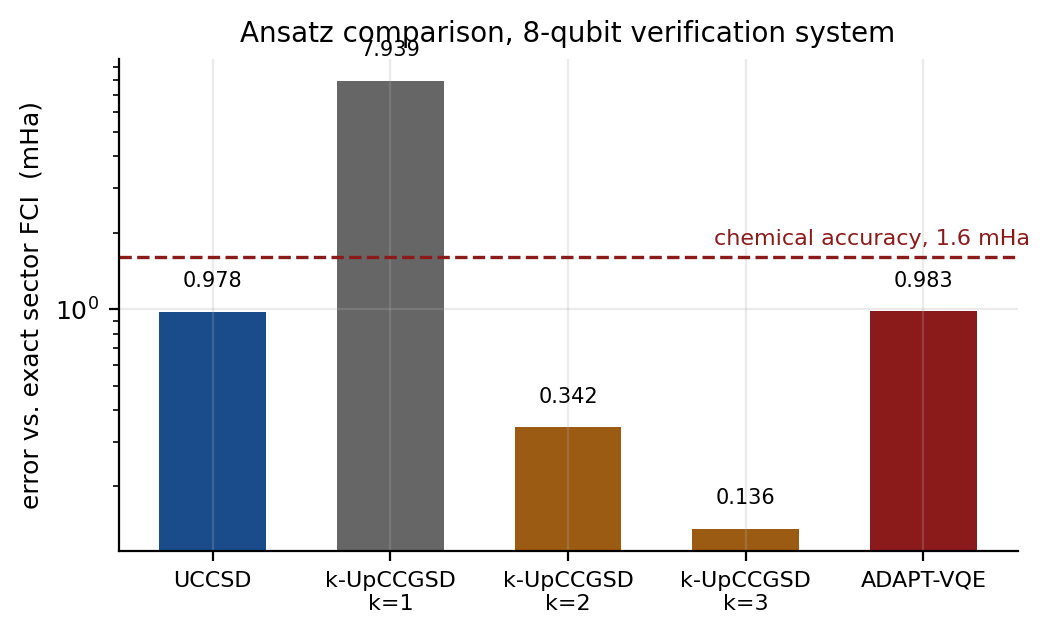
\includegraphics[width=0.72\textwidth]{figures/acr-ansatz.png}
\caption{Error against exact sector FCI, logarithmic. Every configuration except
$k$-UpCCGSD at $k{=}1$ clears chemical accuracy on this system.}
\label{fig:ansatz}
\end{figure}

\begin{figure}[htbp]
\centering
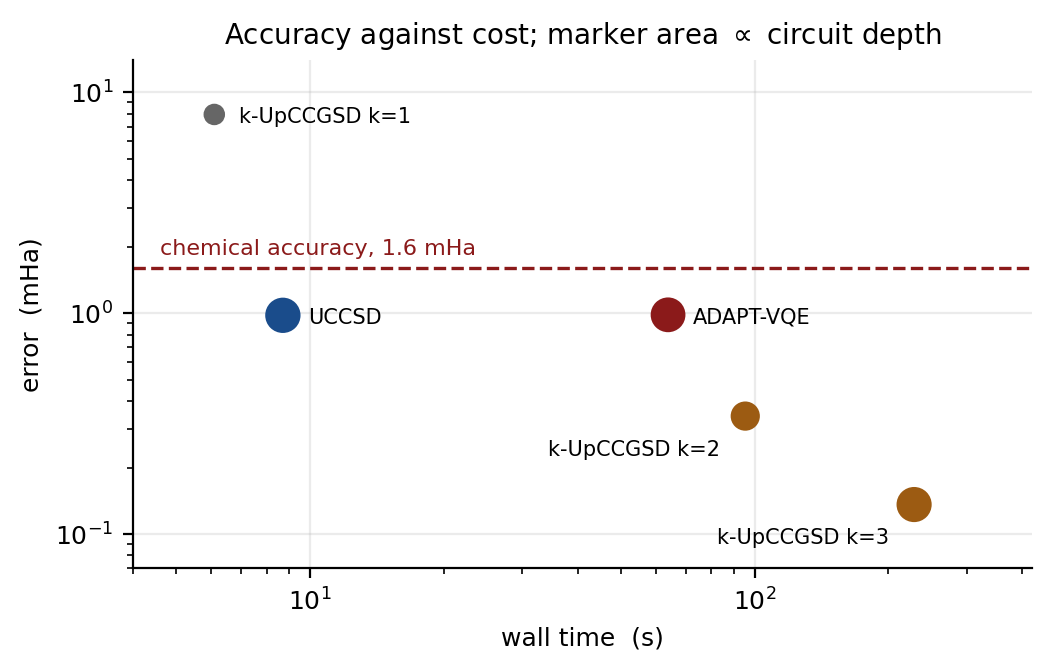
\includegraphics[width=0.72\textwidth]{figures/acr-cost.png}
\caption{The same five runs as accuracy against wall time; marker area is
proportional to circuit depth. UCCSD occupies the corner: within a factor of
three of the best accuracy, at one twenty-sixth of the cost.}
\label{fig:acrcost}
\end{figure}

Two results are worth separating.

\textbf{$k$-UpCCGSD at $k \geq 2$ is more accurate than UCCSD}, by a factor of
$2.9$ at $k{=}2$ and $7.2$ at $k{=}3$. The reason is structural: its excitations
are \emph{generalized}, not restricted to occupied $\to$ virtual, so it reaches
correlation that singles-and-doubles from the reference determinant cannot. The
cost is not proportional --- $k{=}3$ is $26$ times slower than UCCSD for a
$7.2\times$ accuracy gain --- so UCCSD remains the default at this size and
$k$-UpCCGSD becomes the choice above ten qubits, where UCCSD's $O(N^4)$
parameter count stops being affordable.

\textbf{ADAPT-VQE selected all 26 of 26 pool operators.} It rediscovered UCCSD
exactly, arriving at the same energy to within $0.005\mHa$, having spent $7.3$
times the wall time to do so. This is not a failure of ADAPT; it is a statement
about when ADAPT is worth running. The method earns its cost when the pool is
far larger than the number of operators actually required, so that a
gradient-driven search can skip most of it. At eight qubits with a
singles-and-doubles pool, it is not, and the search is pure overhead. ADAPT is
implemented and available, and \code{--ansatz auto} does not select it.

\section{Cost boundary}

\begin{table}[htbp]
\centering
\caption{Measured UCCSD cost on 8 CPU cores, statevector, with a
molecular-scale observable. ``50 iterations'' is the projected wall time of a
converged VQE.}
\label{tab:uccsdscale}
\small
\begin{tabular}{lrrrrr}
\toprule
Register & Params & Depth & 1 energy & 1 gradient & 50 iterations \\
\midrule
8q (4e,4o)  & $26$  & $1{,}646$  & $0.77$ s & $0.7$ min  & $0.6$ h \\
12q (6e,6o) & $117$ & $11{,}127$ & $0.54$ s & $2.1$ min  & $1.8$ h \\
14q (7e,7o) & $204$ & $22{,}163$ & $2.38$ s & $16.2$ min & $13.5$ h \\
16q (8e,8o) & ---   & ---        & \multicolumn{3}{l}{not reached in ${\sim}20$ min} \\
\bottomrule
\end{tabular}
\end{table}

\begin{table}[htbp]
\centering
\caption{Measured $k$-UpCCGSD ($k{=}2$) cost, same machine, $O(N^4)$ Pauli
count, 50-iteration VQE.}
\label{tab:kupscale}
\small
\begin{tabular}{lrrrrr}
\toprule
Register & Params & Depth & 1 energy & 1 gradient & 50 iterations \\
\midrule
12q & $66$  & $3{,}226$  & $0.23$ s & $31$ s     & $0.43$ h \\
14q & $90$  & $4{,}908$  & $0.69$ s & $124$ s    & $1.7$ h \\
16q & $120$ & $7{,}040$  & $1.91$ s & $459$ s    & $6.4$ h \\
18q & $152$ & $9{,}780$  & $9.33$ s & $2{,}846$ s& $40$ h \\
20q & $190$ & $13{,}054$ & $55.8$ s & $21{,}271$ s& $295$ h \\
\bottomrule
\end{tabular}
\end{table}

\begin{figure}[htbp]
\centering
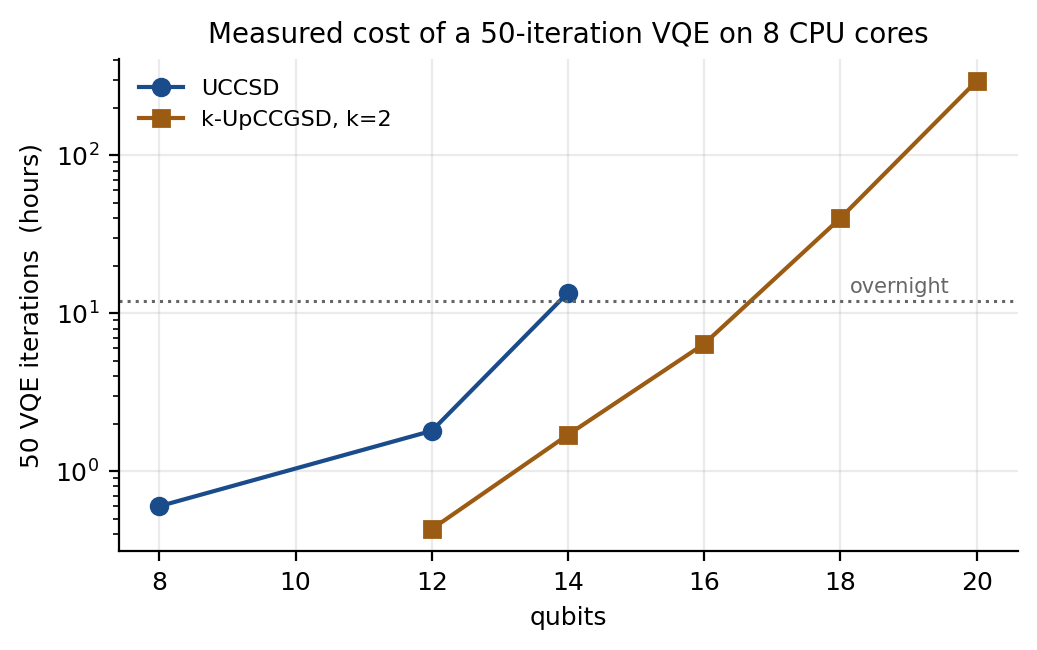
\includegraphics[width=0.72\textwidth]{figures/acr-scaling.png}
\caption{Projected wall time for a 50-iteration VQE against register size, for
both ansatz families. The vertical axis is logarithmic; the curves are steeper
than exponential in qubit count because parameter count and depth grow
simultaneously.}
\label{fig:scaling}
\end{figure}

\begin{result}[The boundary]
The wall is not memory. A 20-qubit statevector is $16$ MB. The cost scales as
(parameters $\times$ depth $\times$ $2^n$ $\times$ terms), and on this workflow
every one of those four factors grows with register size at once. \textbf{16
qubits is the practical ceiling on a laptop; 20 is out of reach.}
\end{result}

For UCCSD specifically, depth roughly doubles per two qubits while parameter
count grows as $O(N^4)$, so gradient cost compounds in both directions: 8q and
12q are comfortable, 14q is an overnight run, and 16q was not reached to
completion.

\section{Implementation findings}

Each of the following was measured, and each overturned the assumption the
workflow was originally written under.

\subsection{Parameter binding is worth $31.5\times$}

Binding parameters with \code{assign\_parameters} costs $419$ ms per circuit,
because each of the 26 UCCSD parameters appears in roughly eight gates as a
symbolic expression evaluated in Python. The Aer execution itself costs $66$ ms.
Handing Aer the unbound circuit plus a bind table moves the work into C++:

\begin{center}
\small
\begin{tabular}{lrrr}
\toprule
53-vector gradient batch & build & run & total \\
\midrule
\code{assign\_parameters} & $33.55$ s & $9.18$ s & $42.73$ s \\
\code{parameter\_binds}   & $0.04$ s  & $1.32$ s & $\mathbf{1.36}$ s \\
\bottomrule
\end{tabular}
\end{center}

Results agree to $3.9\times10^{-14}$. End to end this took the self-test VQE from
$407$ s to $47$ s.

\subsection{Parallelism is method-dependent, and the obvious answer is wrong}

\begin{center}
\small
\begin{tabular}{lrr}
\toprule
& threads $=1$, experiments $=8$ & threads $=8$, experiments $=1$ \\
\midrule
statevector & $70.8$ ms/circuit & $\mathbf{36.0}$ ms \\
MPS         & $\mathbf{83.9}$ ms & $153.9$ ms \\
\bottomrule
\end{tabular}
\end{center}

A shallow circuit is too small to thread, so circuit-level parallelism wins; a
deep one threads well. UCCSD is deep. Defaults are set per method accordingly.

\subsection{Statevector beats MPS here, as predicted}

UCCSD's $1{,}376$ entangling gates saturate the bond dimension --- at eight
qubits $\chi \leq 2^{n/2} = 16$ --- so MPS compresses nothing and pays pure
overhead, losing by $2.3\times$. \textbf{The MPS memory knob is ansatz depth,
not qubit count.} MPS remains the method that scales for weakly entangled
circuits at larger $n$, and the converged energy is cross-checked against exact
statevector either way.

\subsection{Parameter shift is invalid for UCCSD}

Each UCCSD parameter drives roughly eight rotations, so the two-term shift rule
silently returns a wrong gradient. \code{parameter\_shift\_is\_exact()} detects
the condition and refuses. The textbook alternative --- qiskit-algorithms'
adjoint \code{ReverseEstimatorGradient} --- is numerically correct, agreeing with
finite differences to $1.7\times10^{-11}$, but took $619$ s for a single
26-component gradient against $1.36$ s for batched finite differences. It is not
used, and \code{requirements.txt} documents why it is commented out rather than
absent.

\subsection{Aer terminates the process on deep circuits under Windows}

\begin{table}[htbp]
\centering
\caption{Failure is a function of circuit depth, not qubit or gate count.}
\label{tab:crash}
\small
\begin{tabular}{lrrl}
\toprule
Circuit & Gates & Depth & Result \\
\midrule
UCCSD 8q   & $1{,}950$  & $1{,}646$  & fine \\
UCCSD 10q  & $4{,}969$  & $4{,}286$  & fine \\
UCCSD 12q  & $12{,}657$ & $11{,}127$ & \textbf{hard crash, 0xC00000FD} \\
random 12q & $12{,}000$ & $3{,}139$  & fine \\
random 16q & $12{,}000$ & $2{,}390$  & fine \\
\bottomrule
\end{tabular}
\end{table}

The process dies with \code{STACK\_OVERFLOW} and no Python traceback. The cause
is that Aer recurses proportionally to circuit depth while a Windows thread
receives a 1 MB stack against Linux's 8 MB. \code{run\_with\_deep\_stack()} runs
every Aer call on a 64 MB thread, after which the 12-qubit circuit completes in
$0.71$ s. Note that 256 MB and above fail to allocate the thread on Windows, so
the figure is not a knob to raise casually.

\subsection{UCCSD removes the penalty apparatus entirely}

Because UCCSD conserves particle number exactly --- measured leak
$2.8\times10^{-16}$ at the optimum, with no penalty term present --- there is no
penalty to tune, no sector to validate against a penalised operator, no
contamination budget doing work, and no \code{SYMMETRY BROKEN} state reachable.
The hardware-efficient path needs all of it, and on the verification system it
leaves $256\mHa$ of error where UCCSD leaves $0.978\mHa$.

The guarantee is narrower than it is sometimes taken to be: UCCSD conserves $N$
and $S_z$, but \textbf{not} $S^2$ at arbitrary amplitudes, since its
$\alpha\!\to\!\alpha$ and $\beta\!\to\!\beta$ amplitudes are independent. At
random angles the verification system measures $\Ssq = 1.406$. It becomes a spin
eigenstate at the variational minimum --- $\Ssq = 1.12\times10^{-4}$ there ---
which is where the check is applied.

\section{The chemistry that has not been run}
\label{sec:pending}

\begin{unsupported}[No molecular results are reported]
No Hamiltonian has been built for either the \code{ts} or the \code{far}
geometry. This report contains no energy for acrylamide plus methanethiolate, no
TS$-$FAR difference, and no comparison against a classical ladder for this
system. Every number above is either from the verification system or from a
timing measurement.
\end{unsupported}

\subsection{Why}

Building the active-space Hamiltonian requires PySCF, for the restricted
Hartree--Fock, the C-PCM solvation model, the MP2 natural orbital construction
and the CASCI reference. PySCF publishes \textbf{no Windows wheel}; the only
distribution for this platform is a source tarball, and its build is unsupported
on Windows even with a toolchain present. This was confirmed on the machine used
for this report: \code{pip} resolves \code{pyscf-2.14.0.tar.gz} and no binary
distribution, and no WSL distribution is installed to run it under.

The workflow was designed for this constraint rather than blocked by it. The
expensive chemistry is a one-time step whose output is a JSON cache carrying a
specification hash; every downstream command reads the cache and runs natively
on Windows. The split is exactly two commands:

\begin{center}
\small
\begin{tabular}{lll}
\toprule
Command & Requires & Runs on \\
\midrule
\code{prepare}, \code{ladder} & PySCF & Colab / WSL / Linux / macOS \\
\code{validate} & OpenFermion, SciPy & anywhere \\
\code{selftest}, \code{backend}, \code{vqe} & Qiskit, Aer & Windows, natively \\
\bottomrule
\end{tabular}
\end{center}

\subsection{What remains}

\begin{enumerate}[leftmargin=1.4em,itemsep=0.2em]

\item Run \code{colab\_prepare.py --active-spaces 8q --geometries ts,far} on a
  free Colab session. This performs both RHF calculations with C-PCM, builds
  MP2 natural orbitals, selects the active space, runs the classical ladder, and
  packages the caches and receipts for download. The dominant cost is CCSD(T) on
  aug-cc-pVDZ on approximately two vCPUs; \code{--skip-ladder} defers it.

\item Validate and run, on any machine: \code{run.py validate} with
  \code{--cache hamiltonian\_ts\_8q.json --number-penalty 0}, then
  \code{run.py vqe} on each of the two caches. At eight qubits with UCCSD the
  projected cost is $0.6$ hours per geometry (Table~\ref{tab:uccsdscale}).

\item Report the TS$-$FAR difference beside the CASCI$-$CCSD(T) gap from the
  ladder. The latter measures how far the chosen active space sits from
  converged chemistry, and is almost always much larger than the VQE's error
  against CASCI --- so quoting the VQE error alone would overstate what the
  calculation establishes.

\end{enumerate}

\subsection{One anticipated obstacle}

A vacuum anion in a fully augmented basis frequently has a \emph{positive} HOMO,
in which case the frontier orbitals describe the diffuse tail of the wavefunction
rather than the C--S reaction region. The active-space guard in \code{prepare}
detects this and refuses to build rather than producing a Hamiltonian for the
wrong physics. MP2 natural orbitals usually resolve it, which is a second reason
the published protocol uses them. If the guard still fires, the remedies in
order are: restrict diffuse functions to the reacting atoms via a per-element
basis dictionary; or override with
\code{--allow-delocalized-active-space} --- and in that case the result must not
be reported as describing the reaction region.

\section{Claims not supported by these data}

\begin{enumerate}[leftmargin=1.4em,itemsep=0.3em]

\item \textbf{Any statement about the thio-Michael reaction.} No molecular
  calculation was performed.

\item \textbf{That the ansatz ordering in Table~\ref{tab:ansatz} transfers to
  the real system.} The verification system is random. Its correlation energy,
  $374.58\mHa$, is roughly an order of magnitude larger than a CAS(4e,4o)
  molecular active space would typically carry, so it is a harder test in
  absolute terms but not a representative one. The ordering is a hypothesis for
  the real system, not a measurement of it.

\item \textbf{That 16 qubits is a universal ceiling.} It is the ceiling for
  this workflow, these two ansatz families, this machine (8 logical cores), and
  a 50-iteration convergence assumption. A different optimiser, a shallower
  ansatz, or a GPU changes it.

\item \textbf{That the TS$-$FAR difference would be a reaction barrier.} The two
  geometries are \emph{rigid}. Their difference is a rigid-scan energy
  difference along an approach coordinate, not a relaxed barrier.

\item \textbf{Anything about hardware feasibility.} Every measurement here is a
  noiseless simulation.

\end{enumerate}

\section{Limitations}

\begin{enumerate}[leftmargin=1.4em,itemsep=0.2em]
\item The verification system is a single random instance at a single seed. The
  checks are exact, so this is adequate for correctness, but the ansatz
  comparison of \S4 is a single sample.
\item Timings in Tables~\ref{tab:uccsdscale} and~\ref{tab:kupscale} beyond 14
  qubits are projections from measured per-gradient costs, not completed runs.
\item The Aer stack finding is specific to Windows and to the Aer version
  pinned in \code{requirements.txt}.
\item Chemical accuracy, once molecular results exist, will mean agreement with
  CASCI for the cached Hamiltonian --- a statement about the solver, not about
  the basis set or the active space.
\end{enumerate}

\section{Conclusions}

\begin{enumerate}[leftmargin=1.4em,itemsep=0.25em]

\item The solver is verified. Twenty checks against exact classical answers
  pass, including a determinant-by-determinant test of spin-orbital ordering
  that no spectral check could replace.

\item On the verification system UCCSD recovers $99.74\%$ of the correlation
  energy at $0.978\mHa$ above exact FCI in $8.7$ seconds, with structurally
  conserved particle number and no penalty term.

\item $k$-UpCCGSD at $k \geq 2$ is more accurate and disproportionately more
  expensive; ADAPT-VQE reproduced UCCSD's operator set exactly and is not
  selected automatically at this size.

\item Five implementation findings are documented, each of which would
  otherwise have produced a wrong answer, a crashed process, or a
  $30\times$ slower one.

\item No chemistry has been run, for a specific and stated reason, and
  \S\ref{sec:pending} gives the three commands and the projected cost that would
  close the gap.

\end{enumerate}

\appendix

\section{Software environment}

Two environments are recorded. The measurement tables of \S4--\S5 were produced
on the first; the verification run reproduced for this report was executed on the
second, and gives $20/20$ on both.

\begin{center}
\small
\begin{tabular}{lll}
\toprule
& Reference environment & Reproduction environment \\
\midrule
Python      & 3.12.13 & 3.13.7 \\
qiskit      & 2.5.2   & 2.3.1 \\
qiskit-aer  & 0.17.2  & 0.17.2 \\
qiskit-nature & 0.8.0 & 0.7.2 \\
OpenFermion & 1.8.1   & 1.8.1 \\
NumPy       & 2.5.2   & 2.4.3 \\
SciPy       & 1.18.0  & 1.17.1 \\
PySCF       & absent  & absent \\
OS          & Windows 11 & Windows 11 \\
\bottomrule
\end{tabular}
\end{center}

qiskit-nature 0.8.0 predates Qiskit 2.x, so the pairing was tested rather than
assumed: UCCSD builds, simulates on Aer, and places $\theta = 0$ exactly on the
Hartree--Fock determinant.

\section{Reproduction}

\begin{verbatim}
uv venv --python 3.12 .venv && .venv\Scripts\activate
uv pip install -r requirements.txt

python run.py selftest
python run.py backend
python -m unittest discover -s tests -v
\end{verbatim}

Then, on a machine with PySCF:

\begin{verbatim}
pip install -q pyscf openfermion "qiskit==2.5.*" \
               "qiskit-aer==0.17.*" "qiskit-nature==0.8.*"
python colab_prepare.py --active-spaces 8q --geometries ts,far
\end{verbatim}

Unzip the resulting archive into the workflow folder, then anywhere:

\begin{verbatim}
python run.py validate --cache hamiltonian_ts_8q.json --number-penalty 0
python run.py vqe      --cache hamiltonian_ts_8q.json
python run.py vqe      --cache hamiltonian_far_8q.json
python run.py ladder
\end{verbatim}

\section{Data inventory}

\begin{center}
\small
\begin{tabular}{ll}
\toprule
Artifact & Status \\
\midrule
\code{report/figures/acr-ansatz.png}   & present, from Table~\ref{tab:ansatz} \\
\code{report/figures/acr-cost.png}     & present, from Table~\ref{tab:ansatz} \\
\code{report/figures/acr-scaling.png}  & present, from Tables~\ref{tab:uccsdscale}--\ref{tab:kupscale} \\
\code{acrylamide\_thiolate\_hamiltonian.json} & \textbf{not built} \\
\code{acrylamide\_thiolate\_vqe\_result.json} & \textbf{not built} \\
\code{acrylamide\_thiolate\_classical\_ladder.json} & \textbf{not built} \\
\bottomrule
\end{tabular}
\end{center}

The three absent files are the entire chemistry output of this workflow. Their
absence is the subject of \S\ref{sec:pending} and is the reason this document is
titled a verification report.

\section*{References}
\small
\begin{enumerate}[leftmargin=1.4em,itemsep=0.1em]
\item CovAngelo, \emph{Covalent inhibitor reaction energetics on quantum
  hardware}, arXiv:2604.10487 --- the simulator protocol followed here, and the
  source of Table~\ref{tab:protocol}.
\item J.\ Lee \emph{et al.}, \emph{Generalized unitary coupled cluster
  wavefunctions for quantum computation}, J.\ Chem.\ Theory Comput.\ \textbf{15},
  311 (2019) --- $k$-UpCCGSD.
\item H.\ R.\ Grimsley \emph{et al.}, \emph{An adaptive variational algorithm
  for exact molecular simulations on a quantum computer}, Nat.\ Commun.\
  \textbf{10}, 3007 (2019) --- ADAPT-VQE.
\end{enumerate}

\end{document}
